% !TeX document-id = {58dd56a7-a545-4332-9f31-aa9515ad78e0}
%%%%%%%%%%%%%%%%%%%%%%%%%%%%%%%%%%%%%%%%%
% The Legrand Orange Book
% LaTeX Template
% Version 2.4 (26/09/2018)
%
% This template was downloaded from:
% http://www.LaTeXTemplates.com
%
% Original author:
% Mathias Legrand (legrand.mathias@gmail.com) with modifications by:
% Vel (vel@latextemplates.com)
%
% License:
% CC BY-NC-SA 3.0 (http://creativecommons.org/licenses/by-nc-sa/3.0/)
%
% Compiling this template:
% This template uses biber for its bibliography and makeindex for its index.
% When you first open the template, compile it from the command line with the 
% commands below to make sure your LaTeX distribution is configured correctly:
%
% 1) pdflatex main
% 2) makeindex main.idx -s StyleInd.ist
% 3) biber main
% 4) pdflatex main x 2
%
% After this, when you wish to update the bibliography/index use the appropriate
% command above and make sure to compile with pdflatex several times 
% afterwards to propagate your changes to the document.
%
% This template also uses a number of packages which may need to be
% updated to the newest versions for the template to compile. It is strongly
% recommended you update your LaTeX distribution if you have any
% compilation errors.
%
% Important note:
% Chapter heading images should have a 2:1 width:height ratio,
% e.g. 920px width and 460px height.
%
%%%%%%%%%%%%%%%%%%%%%%%%%%%%%%%%%%%%%%%%%

%----------------------------------------------------------------------------------------
%	PACKAGES AND OTHER DOCUMENT CONFIGURATIONS
%----------------------------------------------------------------------------------------

% !BIB program = biber
% !TeX TXS-program:compile = txs:///pdflatex/[--shell-escape]

\documentclass[11pt,fleqn]{book} % Default font size and left-justified equations

%%%%%%%%%%%%%%%%%%%%%%%%%%%%%%%%%%%%%%%%%
% The Legrand Orange Book
% Structural Definitions File
% Version 2.1 (26/09/2018)
%
% Original author:
% Mathias Legrand (legrand.mathias@gmail.com) with modifications by:
% Vel (vel@latextemplates.com)
% 
% This file was downloaded from:
% http://www.LaTeXTemplates.com
%
% License:
% CC BY-NC-SA 3.0 (http://creativecommons.org/licenses/by-nc-sa/3.0/)
%
%%%%%%%%%%%%%%%%%%%%%%%%%%%%%%%%%%%%%%%%%

%----------------------------------------------------------------------------------------
%	VARIOUS REQUIRED PACKAGES AND CONFIGURATIONS
%----------------------------------------------------------------------------------------

\usepackage{graphicx} % Required for including pictures
\graphicspath{{assets/}} % Specifies the directory where pictures are stored

\usepackage{lipsum} % Inserts dummy text

\usepackage{tikz} % Required for drawing custom shapes

\usepackage[dutch]{babel} % English language/hyphenation

\usepackage{enumitem} % Customize lists
\setlist{nolistsep} % Reduce spacing between bullet points and numbered lists

\usepackage{booktabs} % Required for nicer horizontal rules in tables

\usepackage{xcolor} % Required for specifying colors by name
\definecolor{ocre}{RGB}{22,57,123} % Define the orange color used for highlighting throughout the book

%----------------------------------------------------------------------------------------
%	MARGINS
%----------------------------------------------------------------------------------------

\usepackage{geometry} % Required for adjusting page dimensions and margins

\geometry{
	paper=a4paper, % Paper size, change to letterpaper for US letter size
	top=3cm, % Top margin
	bottom=3cm, % Bottom margin
	left=3cm, % Left margin
	right=3cm, % Right margin
	headheight=14pt, % Header height
	footskip=1.4cm, % Space from the bottom margin to the baseline of the footer
	headsep=10pt, % Space from the top margin to the baseline of the header
	%showframe, % Uncomment to show how the type block is set on the page
}

%----------------------------------------------------------------------------------------
%	FONTS
%----------------------------------------------------------------------------------------

\usepackage{avant} % Use the Avantgarde font for headings
%\usepackage{times} % Use the Times font for headings
%\usepackage{helvet}
%\usepackage{mathptmx} % Use the Adobe Times Roman as the default text font together with math symbols from the Sym­bol, Chancery and Com­puter Modern fonts

\usepackage{microtype} % Slightly tweak font spacing for aesthetics
\usepackage[utf8]{inputenc} % Required for including letters with accents
\usepackage[T1]{fontenc} % Use 8-bit encoding that has 256 glyphs
\renewcommand{\familydefault}{cmss}

%----------------------------------------------------------------------------------------
%	BIBLIOGRAPHY AND INDEX
%----------------------------------------------------------------------------------------

\usepackage[style=numeric,citestyle=numeric,sorting=nyt,sortcites=true,autopunct=true,babel=hyphen,hyperref=true,abbreviate=false,backref=true,backend=biber]{biblatex}
\addbibresource{bibliography.bib} % BibTeX bibliography file
\defbibheading{bibempty}{}

\usepackage{calc} % For simpler calculation - used for spacing the index letter headings correctly
\usepackage{makeidx} % Required to make an index
\makeindex % Tells LaTeX to create the files required for indexing

%----------------------------------------------------------------------------------------
%	MAIN TABLE OF CONTENTS
%----------------------------------------------------------------------------------------

\usepackage{titletoc} % Required for manipulating the table of contents

\contentsmargin{0cm} % Removes the default margin

% Part text styling (this is mostly taken care of in the PART HEADINGS section of this file)
\titlecontents{part}
	[0cm] % Left indentation
	{\addvspace{20pt}\bfseries} % Spacing and font options for parts
	{}
	{}
	{}

% Chapter text styling
\titlecontents{chapter}
	[1.25cm] % Left indentation
	{\addvspace{12pt}\large\sffamily\bfseries} % Spacing and font options for chapters
	{\color{ocre!60}\contentslabel[\Large\thecontentslabel]{1.25cm}\color{ocre}} % Formatting of numbered sections of this type
	{\color{ocre}} % Formatting of numberless sections of this type
	{\color{ocre!60}\normalsize\;\titlerule*[.5pc]{.}\;\thecontentspage} % Formatting of the filler to the right of the heading and the page number

% Section text styling
\titlecontents{section}
	[1.25cm] % Left indentation
	{\addvspace{3pt}\sffamily\bfseries} % Spacing and font options for sections
	{\contentslabel[\thecontentslabel]{1.25cm}} % Formatting of numbered sections of this type
	{} % Formatting of numberless sections of this type
	{\hfill\color{black}\thecontentspage} % Formatting of the filler to the right of the heading and the page number

% Subsection text styling
\titlecontents{subsection}
	[1.25cm] % Left indentation
	{\addvspace{1pt}\sffamily\small} % Spacing and font options for subsections
	{\contentslabel[\thecontentslabel]{1.25cm}} % Formatting of numbered sections of this type
	{} % Formatting of numberless sections of this type
	{\ \titlerule*[.5pc]{.}\;\thecontentspage} % Formatting of the filler to the right of the heading and the page number

% Figure text styling
\titlecontents{figure}
	[1.25cm] % Left indentation
	{\addvspace{1pt}\sffamily\small} % Spacing and font options for figures
	{\thecontentslabel\hspace*{1em}} % Formatting of numbered sections of this type
	{} % Formatting of numberless sections of this type
	{\ \titlerule*[.5pc]{.}\;\thecontentspage} % Formatting of the filler to the right of the heading and the page number

% Table text styling
\titlecontents{table}
	[1.25cm] % Left indentation
	{\addvspace{1pt}\sffamily\small} % Spacing and font options for tables
	{\thecontentslabel\hspace*{1em}} % Formatting of numbered sections of this type
	{} % Formatting of numberless sections of this type
	{\ \titlerule*[.5pc]{.}\;\thecontentspage} % Formatting of the filler to the right of the heading and the page number

%----------------------------------------------------------------------------------------
%	MINI TABLE OF CONTENTS IN PART HEADS
%----------------------------------------------------------------------------------------

% Chapter text styling
\titlecontents{lchapter}
	[0em] % Left indentation
	{\addvspace{15pt}\large\sffamily\bfseries} % Spacing and font options for chapters
	{\color{ocre}\contentslabel[\Large\thecontentslabel]{1.25cm}\color{ocre}} % Chapter number
	{}  
	{\color{ocre}\normalsize\sffamily\bfseries\;\titlerule*[.5pc]{.}\;\thecontentspage} % Page number

% Section text styling
\titlecontents{lsection}
	[0em] % Left indentation
	{\sffamily\small} % Spacing and font options for sections
	{\contentslabel[\thecontentslabel]{1.25cm}} % Section number
	{}
	{}

% Subsection text styling (note these aren't shown by default, display them by searchings this file for tocdepth and reading the commented text)
\titlecontents{lsubsection}
	[.5em] % Left indentation
	{\sffamily\footnotesize} % Spacing and font options for subsections
	{\contentslabel[\thecontentslabel]{1.25cm}}
	{}
	{}

%----------------------------------------------------------------------------------------
%	HEADERS AND FOOTERS
%----------------------------------------------------------------------------------------

\usepackage{fancyhdr} % Required for header and footer configuration

\pagestyle{fancy} % Enable the custom headers and footers

\renewcommand{\chaptermark}[1]{\markboth{\sffamily\normalsize\bfseries\chaptername\ \thechapter.\ #1}{}} % Styling for the current chapter in the header
\renewcommand{\sectionmark}[1]{\markright{\sffamily\normalsize\thesection\hspace{5pt}#1}{}} % Styling for the current section in the header

\fancyhf{} % Clear default headers and footers
\fancyhead[LE,RO]{\sffamily\normalsize\thepage} % Styling for the page number in the header
\fancyhead[LO]{\rightmark} % Print the nearest section name on the left side of odd pages
\fancyhead[RE]{\leftmark} % Print the current chapter name on the right side of even pages
%\fancyfoot[C]{\thepage} % Uncomment to include a footer

\renewcommand{\headrulewidth}{0.5pt} % Thickness of the rule under the header

\fancypagestyle{plain}{% Style for when a plain pagestyle is specified
	\fancyhead{}\renewcommand{\headrulewidth}{0pt}%
}

% Removes the header from odd empty pages at the end of chapters
\makeatletter
\renewcommand{\cleardoublepage}{
\clearpage\ifodd\c@page\else
\hbox{}
\vspace*{\fill}
\thispagestyle{empty}
\newpage
\fi}

%----------------------------------------------------------------------------------------
%	THEOREM STYLES
%----------------------------------------------------------------------------------------

\usepackage{amsmath,amsfonts,amssymb,amsthm} % For math equations, theorems, symbols, etc

\newcommand{\intoo}[2]{\mathopen{]}#1\,;#2\mathclose{[}}
\newcommand{\ud}{\mathop{\mathrm{{}d}}\mathopen{}}
\newcommand{\intff}[2]{\mathopen{[}#1\,;#2\mathclose{]}}
\renewcommand{\qedsymbol}{$\blacksquare$}
\newtheorem{notation}{Notation}[chapter]

% Boxed/framed environments
\newtheoremstyle{ocrenumbox}% Theorem style name
{0pt}% Space above
{0pt}% Space below
{\normalfont}% Body font
{}% Indent amount
{\small\bf\sffamily\color{ocre}}% Theorem head font
{\;}% Punctuation after theorem head
{0.25em}% Space after theorem head
{\small\sffamily\color{ocre}\thmname{#1}\nobreakspace\thmnumber{\@ifnotempty{#1}{}\@upn{#2}}% Theorem text (e.g. Theorem 2.1)
\thmnote{\nobreakspace\the\thm@notefont\sffamily\bfseries\color{black}---\nobreakspace#3.}} % Optional theorem note

\newtheoremstyle{blacknumex}% Theorem style name
{5pt}% Space above
{5pt}% Space below
{\normalfont}% Body font
{} % Indent amount
{\small\bf\sffamily}% Theorem head font
{\;}% Punctuation after theorem head
{0.25em}% Space after theorem head
{\small\sffamily{\tiny\ensuremath{\blacksquare}}\nobreakspace\thmname{#1}\nobreakspace\thmnumber{\@ifnotempty{#1}{}\@upn{#2}}% Theorem text (e.g. Theorem 2.1)
\thmnote{\nobreakspace\the\thm@notefont\sffamily\bfseries---\nobreakspace#3.}}% Optional theorem note

\newtheoremstyle{blacknumbox} % Theorem style name
{0pt}% Space above
{0pt}% Space below
{\normalfont}% Body font
{}% Indent amount
{\small\bf\sffamily}% Theorem head font
{\;}% Punctuation after theorem head
{0.25em}% Space after theorem head
{\small\sffamily\thmname{#1}\nobreakspace\thmnumber{\@ifnotempty{#1}{}\@upn{#2}}% Theorem text (e.g. Theorem 2.1)
\thmnote{\nobreakspace\the\thm@notefont\sffamily\bfseries---\nobreakspace#3.}}% Optional theorem note

% Non-boxed/non-framed environments
\newtheoremstyle{ocrenum}% Theorem style name
{5pt}% Space above
{5pt}% Space below
{\normalfont}% Body font
{}% Indent amount
{\small\bf\sffamily\color{ocre}}% Theorem head font
{\;}% Punctuation after theorem head
{0.25em}% Space after theorem head
{\small\sffamily\color{ocre}\thmname{#1}\nobreakspace\thmnumber{\@ifnotempty{#1}{}\@upn{#2}}% Theorem text (e.g. Theorem 2.1)
\thmnote{\nobreakspace\the\thm@notefont\sffamily\bfseries\color{black}---\nobreakspace#3.}} % Optional theorem note
\makeatother

% Defines the theorem text style for each type of theorem to one of the three styles above
\newcounter{dummy} 
\numberwithin{dummy}{section}
\theoremstyle{ocrenumbox}
\newtheorem{theoremeT}[dummy]{Theorem}
\newtheorem{problem}{Probleem}[chapter]
\newtheorem{exerciseT}{Oefening}[chapter]
\theoremstyle{blacknumex}
\newtheorem{exampleT}{Voorbeeld}[chapter]
\theoremstyle{blacknumbox}
\newtheorem{vocabulary}{Vocabulaire}[chapter]
\newtheorem{definitionT}{Definitie}[section]
\newtheorem{corollaryT}[dummy]{Gevolg}
\theoremstyle{ocrenum}
\newtheorem{proposition}[dummy]{Propositie}

% Library function description
\theoremstyle{ocrenumbox}
\newtheorem*{libfT}{Library}

%----------------------------------------------------------------------------------------
%	DEFINITION OF COLORED BOXES
%----------------------------------------------------------------------------------------

\RequirePackage[framemethod=default]{mdframed} % Required for creating the theorem, definition, exercise and corollary boxes

% Theorem box
\newmdenv[skipabove=7pt,
skipbelow=7pt,
backgroundcolor=black!5,
linecolor=ocre,
innerleftmargin=5pt,
innerrightmargin=5pt,
innertopmargin=5pt,
leftmargin=0cm,
rightmargin=0cm,
innerbottommargin=5pt]{tBox}

% Exercise box	  
\newmdenv[skipabove=7pt,
skipbelow=7pt,
rightline=false,
leftline=true,
topline=false,
bottomline=false,
backgroundcolor=ocre!10,
linecolor=ocre,
innerleftmargin=5pt,
innerrightmargin=5pt,
innertopmargin=5pt,
innerbottommargin=5pt,
leftmargin=0cm,
rightmargin=0cm,
linewidth=4pt]{eBox}	

% Definition box
\newmdenv[skipabove=7pt,
skipbelow=7pt,
rightline=false,
leftline=true,
topline=false,
bottomline=false,
linecolor=ocre,
innerleftmargin=5pt,
innerrightmargin=5pt,
innertopmargin=0pt,
leftmargin=0cm,
rightmargin=0cm,
linewidth=4pt,
innerbottommargin=0pt]{dBox}	

% Corollary box
\newmdenv[skipabove=7pt,
skipbelow=7pt,
rightline=false,
leftline=true,
topline=false,
bottomline=false,
linecolor=gray,
backgroundcolor=black!5,
innerleftmargin=5pt,
innerrightmargin=5pt,
innertopmargin=5pt,
leftmargin=0cm,
rightmargin=0cm,
linewidth=4pt,
innerbottommargin=5pt]{cBox}

% Creates an environment for each type of theorem and assigns it a theorem text style from the "Theorem Styles" section above and a colored box from above
\newenvironment{theorem}{\begin{tBox}\begin{theoremeT}}{\end{theoremeT}\end{tBox}}
\newenvironment{exercise}{\begin{eBox}\begin{exerciseT}}{\hfill{\color{ocre}\tiny\ensuremath{\blacktriangleleft}}\end{exerciseT}\end{eBox}}				  
\newenvironment{definition}{\begin{dBox}\begin{definitionT}}{\end{definitionT}\end{dBox}}	
\newenvironment{example}{\begin{exampleT}}{\hfill{\tiny\ensuremath{\blacktriangleleft}}\end{exampleT}}		
\newenvironment{corollary}{\begin{cBox}\begin{corollaryT}}{\end{corollaryT}\end{cBox}}	

\newenvironment{libf}{\begin{tBox}\begin{libfT}}{\end{libfT}\end{tBox}}

%----------------------------------------------------------------------------------------
%	REMARK ENVIRONMENT
%----------------------------------------------------------------------------------------

\newenvironment{remark}{\par\vspace{10pt}\small % Vertical white space above the remark and smaller font size
\begin{list}{}{
\leftmargin=35pt % Indentation on the left
\rightmargin=25pt}\item\ignorespaces % Indentation on the right
\makebox[-2.5pt]{\begin{tikzpicture}[overlay]
\node[draw=ocre!60,line width=1pt,circle,fill=ocre!25,font=\sffamily\bfseries,inner sep=2pt,outer sep=0pt] at (-15pt,0pt){\textcolor{ocre}{$\bigstar$}};\end{tikzpicture}} % Orange R in a circle
\advance\baselineskip -1pt}{\end{list}\vskip5pt} % Tighter line spacing and white space after remark

%----------------------------------------------------------------------------------------
%	SECTION NUMBERING IN THE MARGIN
%----------------------------------------------------------------------------------------

\makeatletter
\renewcommand{\@seccntformat}[1]{\llap{\textcolor{ocre}{\csname the#1\endcsname}\hspace{1em}}}                    
\renewcommand{\section}{\@startsection{section}{1}{\z@}
{-4ex \@plus -1ex \@minus -.4ex}
{1ex \@plus.2ex }
{\normalfont\large\sffamily\bfseries}}
\renewcommand{\subsection}{\@startsection {subsection}{2}{\z@}
{-3ex \@plus -0.1ex \@minus -.4ex}
{0.5ex \@plus.2ex }
{\normalfont\sffamily\bfseries}}
\renewcommand{\subsubsection}{\@startsection {subsubsection}{3}{\z@}
{-2ex \@plus -0.1ex \@minus -.2ex}
{.2ex \@plus.2ex }
{\normalfont\small\sffamily\bfseries}}                        
\renewcommand\paragraph{\@startsection{paragraph}{4}{\z@}
{-2ex \@plus-.2ex \@minus .2ex}
{.1ex}
{\normalfont\small\sffamily\bfseries}}

%----------------------------------------------------------------------------------------
%	PART HEADINGS
%----------------------------------------------------------------------------------------

% Numbered part in the table of contents
\newcommand{\@mypartnumtocformat}[2]{%
	\setlength\fboxsep{0pt}%
	\noindent\colorbox{ocre!20}{\strut\parbox[c][.7cm]{\ecart}{\color{ocre!70}\Large\sffamily\bfseries\centering#1}}\hskip\esp\colorbox{ocre!40}{\strut\parbox[c][.7cm]{\linewidth-\ecart-\esp}{\Large\sffamily\centering#2}}%
}

% Unnumbered part in the table of contents
\newcommand{\@myparttocformat}[1]{%
	\setlength\fboxsep{0pt}%
	\noindent\colorbox{ocre!40}{\strut\parbox[c][.7cm]{\linewidth}{\Large\sffamily\centering#1}}%
}

\newlength\esp
\setlength\esp{4pt}
\newlength\ecart
\setlength\ecart{1.2cm-\esp}
\newcommand{\thepartimage}{}%
\newcommand{\partimage}[1]{\renewcommand{\thepartimage}{#1}}%
\def\@part[#1]#2{%
\ifnum \c@secnumdepth >-2\relax%
\refstepcounter{part}%
\addcontentsline{toc}{part}{\texorpdfstring{\protect\@mypartnumtocformat{\thepart}{#1}}{\partname~\thepart\ ---\ #1}}
\else%
\addcontentsline{toc}{part}{\texorpdfstring{\protect\@myparttocformat{#1}}{#1}}%
\fi%
\startcontents%
\markboth{}{}%
{\thispagestyle{empty}%
\begin{tikzpicture}[remember picture,overlay]%
\node at (current page.north west){\begin{tikzpicture}[remember picture,overlay]%	
\fill[ocre!20](0cm,0cm) rectangle (\paperwidth,-\paperheight);
\node[anchor=north] at (4cm,-3.25cm){\color{ocre!40}\fontsize{220}{100}\sffamily\bfseries\thepart}; 
\node[anchor=south east] at (\paperwidth-1cm,-\paperheight+1cm){\parbox[t][][t]{8.5cm}{
\printcontents{l}{0}{\setcounter{tocdepth}{1}}% The depth to which the Part mini table of contents displays headings; 0 for chapters only, 1 for chapters and sections and 2 for chapters, sections and subsections
}};
\node[anchor=north east] at (\paperwidth-1.5cm,-3.25cm){\parbox[t][][t]{15cm}{\strut\raggedleft\color{white}\fontsize{30}{30}\sffamily\bfseries#2}};
\end{tikzpicture}};
\end{tikzpicture}}%
\@endpart}
\def\@spart#1{%
\startcontents%
\phantomsection
{\thispagestyle{empty}%
\begin{tikzpicture}[remember picture,overlay]%
\node at (current page.north west){\begin{tikzpicture}[remember picture,overlay]%	
\fill[ocre!20](0cm,0cm) rectangle (\paperwidth,-\paperheight);
\node[anchor=north east] at (\paperwidth-1.5cm,-3.25cm){\parbox[t][][t]{15cm}{\strut\raggedleft\color{white}\fontsize{30}{30}\sffamily\bfseries#1}};
\end{tikzpicture}};
\end{tikzpicture}}
\addcontentsline{toc}{part}{\texorpdfstring{%
\setlength\fboxsep{0pt}%
\noindent\protect\colorbox{ocre!40}{\strut\protect\parbox[c][.7cm]{\linewidth}{\Large\sffamily\protect\centering #1\quad\mbox{}}}}{#1}}%
\@endpart}
\def\@endpart{\vfil\newpage
\if@twoside
\if@openright
\null
\thispagestyle{empty}%
\newpage
\fi
\fi
\if@tempswa
\twocolumn
\fi}

%----------------------------------------------------------------------------------------
%	CHAPTER HEADINGS
%----------------------------------------------------------------------------------------

% A switch to conditionally include a picture, implemented by Christian Hupfer
\newif\ifusechapterimage
\usechapterimagetrue
\newcommand{\thechapterimage}{}%
\newcommand{\chapterimage}[1]{\ifusechapterimage\renewcommand{\thechapterimage}{#1}\fi}%
\newcommand{\autodot}{.}
\def\@makechapterhead#1{%
{\parindent \z@ \raggedright \normalfont
\ifnum \c@secnumdepth >\m@ne
\if@mainmatter
\begin{tikzpicture}[remember picture,overlay]
\node at (current page.north west)
{\begin{tikzpicture}[remember picture,overlay]
\node[anchor=north west,inner sep=0pt] at (0,0) {\ifusechapterimage\includegraphics[width=\paperwidth]{\thechapterimage}\fi};
\draw[anchor=west] (\Gm@lmargin,-9cm) node [line width=2pt,rounded corners=15pt,draw=ocre,fill=white,fill opacity=0.8,inner sep=15pt]{\strut\makebox[22cm]{}};
\draw[anchor=west] (\Gm@lmargin+.3cm,-9cm) node {\huge\sffamily\bfseries\color{black}\thechapter\autodot~#1\strut};
\end{tikzpicture}};
\end{tikzpicture}
\else
\begin{tikzpicture}[remember picture,overlay]
\node at (current page.north west)
{\begin{tikzpicture}[remember picture,overlay]
\node[anchor=north west,inner sep=0pt] at (0,0) {\ifusechapterimage\includegraphics[width=\paperwidth]{\thechapterimage}\fi};
\draw[anchor=west] (\Gm@lmargin,-9cm) node [line width=2pt,rounded corners=15pt,draw=ocre,fill=white,fill opacity=0.8,inner sep=15pt]{\strut\makebox[22cm]{}};
\draw[anchor=west] (\Gm@lmargin+.3cm,-9cm) node {\huge\sffamily\bfseries\color{black}#1\strut};
\end{tikzpicture}};
\end{tikzpicture}
\fi\fi\par\vspace*{270\p@}}}

%-------------------------------------------

\def\@makeschapterhead#1{%
\begin{tikzpicture}[remember picture,overlay]
\node at (current page.north west)
{\begin{tikzpicture}[remember picture,overlay]
\node[anchor=north west,inner sep=0pt] at (0,0) {\ifusechapterimage\includegraphics[width=\paperwidth]{\thechapterimage}\fi};
\draw[anchor=west] (\Gm@lmargin,-9cm) node [line width=2pt,rounded corners=15pt,draw=ocre,fill=white,fill opacity=0.8,inner sep=15pt]{\strut\makebox[22cm]{}};
\draw[anchor=west] (\Gm@lmargin+.3cm,-9cm) node {\huge\sffamily\bfseries\color{black}#1\strut};
\end{tikzpicture}};
\end{tikzpicture}
\par\vspace*{270\p@}}
\makeatother

%----------------------------------------------------------------------------------------
%	LINKS
%----------------------------------------------------------------------------------------

\usepackage{hyperref}
\hypersetup{hidelinks,backref=true,pagebackref=true,hyperindex=true,colorlinks=false,breaklinks=true,urlcolor=ocre,bookmarks=true,bookmarksopen=false}

\usepackage{bookmark}
\bookmarksetup{
open,
numbered,
addtohook={%
\ifnum\bookmarkget{level}=0 % chapter
\bookmarksetup{bold}%
\fi
\ifnum\bookmarkget{level}=-1 % part
\bookmarksetup{color=ocre,bold}%
\fi
}
}


%--------
%  CODE
%--------

\usepackage{minted}

\usepackage{todonotes}
\usepackage{multicol}
\usepackage{wrapfig} % Insert the commands.tex file which contains the majority of the structure behind the template

\hypersetup{pdftitle={Arduboy Starters Guide},pdfauthor={Stijn Caerts}} % Uncomment and fill out to include PDF metadata for the author and title of the book

\usepackage[scale=2]{ccicons}

\def\Cpp{{C\nolinebreak[4]\hspace{-.05em}\raisebox{.4ex}{\tiny\bf ++}}}

%----------------------------------------------------------------------------------------

\begin{document}

%----------------------------------------------------------------------------------------
%	TITLE PAGE
%----------------------------------------------------------------------------------------

\begingroup
\thispagestyle{empty} % Suppress headers and footers on the title page
\begin{tikzpicture}[remember picture,overlay]
\node[inner sep=0pt] (background) at (current page.center) {
\includegraphics[width=\paperwidth]{jcw_background.pdf}};
\draw (current page.center) node [fill=ocre!30!white,fill opacity=0.9,text opacity=1,inner sep=1cm]{\Huge\centering\bfseries\sffamily\parbox[c][][t]{\paperwidth}{\centering Arduboy\\[15pt] % Book title
{\Large Starters Guide}\\[20pt] % Subtitle
{\huge Stijn Caerts}}}; % Author name

\node[yshift=2cm] at (current page.south){
\includegraphics[height=3cm]{jcw_logo.pdf}};
\end{tikzpicture}
\vfill
\endgroup

%----------------------------------------------------------------------------------------
%	COPYRIGHT PAGE
%----------------------------------------------------------------------------------------

\newpage
~\vfill
\thispagestyle{empty}
{
\fontfamily{ptm}\selectfont

\noindent Copyright \copyright\ 2019 Stijn Caerts\\ % Copyright notice

\noindent \textsc{Jeugd, Cultuur en Wetenschap vzw}\\ % Publisher

\noindent \textsc{\href{https://stijn.caerts.be/}{stijn.caerts.be}} -- \textsc{\href{https://www.jeugdcultuurenwetenschap.be/}{www.jeugdcultuurenwetenschap.be}}\\ % URL

\noindent Dit werk valt onder een \href{https://creativecommons.org/licenses/by-nc-sa/4.0/deed.nl}{Creative Commons Naamsvermelding-NietCommercieel-GelijkDelen 4.0 Internationaal-licentie} (de ``Licentie''). Dit document mag enkel gebruikt worden in navolging van de Licentie. De volledige Licentie-tekst is beschikbaar op \url{https://creativecommons.org/licenses/by-nc-sa/4.0/}.\\

\noindent \href{https://creativecommons.org/licenses/by-nc-sa/4.0/}{\ccbyncsaeu}

\vspace{1cm}

\noindent \textit{Eerste versie, augustus 2019} % Printing/edition date
}

%----------------------------------------------------------------------------------------
%	TABLE OF CONTENTS
%----------------------------------------------------------------------------------------

%\usechapterimagefalse % If you don't want to include a chapter image, use this to toggle images off - it can be enabled later with \usechapterimagetrue

\chapterimage{jcw_header.pdf} % Table of contents heading image

\pagestyle{empty} % Disable headers and footers for the following pages

\tableofcontents % Print the table of contents itself

\cleardoublepage % Forces the first chapter to start on an odd page so it's on the right side of the book

\pagestyle{fancy} % Enable headers and footers again

%----------------------------------------------------------------------------------------
%	PART
%----------------------------------------------------------------------------------------

\part{Introductie tot C++}
\chapterimage{jcw_header.pdf}
\chapter{Inleiding}
\section{Wat is C++?}
% https://www.tutorialspoint.com/cplusplus
Programma's voor \textbf{Arduino} en \textbf{Arduboy} worden geschreven in de programmeertaal \Cpp\index{C++@\Cpp}. Het is niet nodig om de hele programmeertaal te kennen en begrijpen voor je aan de slag kan gaan met programmeren. Daarom geven we hier een beknopt overzicht van de belangrijkste concepten die je nodig hebt om van start te gaan.\\

\noindent In de volgende hoofdstukken komen variabelen en types, controlestructuren (if-then-else, for, while) en functies en procedures aan bod. Tot slot zijn er nog twee hoofdstukken die dieper ingaan op de mogelijkheden van \Cpp, namelijk arrays en lijsten, en klassen en objecten.\\

\noindent Voor een interactieve en uitgebreidere introductie tot \Cpp, kan je terecht bij W3Schools (\url{https://www.w3schools.com/cpp/}).

\nocite{w3schools:cpp, tutorialspoint:cpp}

\section{Syntax}
\subsection{Puntkomma}
\index{Puntkomma}
Achter elke instructie wordt in \Cpp{} een puntkomma \mintinline{cpp}{;} geplaatst. Deze puntkomma vertelt de compiler dat op die plaats een instructie eindigt. Als je een puntkomma vergeet te plaatsen, is het programma niet correct en zal je het programma niet kunnen compileren. De compiler zal dan een foutmelding geven.

\subsection{Accolades}
\index{Accolade}
Accolades \mintinline{cpp}{{}} worden gebruikt om een blok code aan te duiden. De accolades moeten gebalanceerd voorkomen in de code, wat betekent dat voor elke openende accolade \texttt{\{} er een bijhorende sluitende accolade \texttt{\}} moet zijn. Het gebruik van accolades wordt later geïllustreerd bij de controlestructuren (if-then-else, for, ..), functies en klassen.

\subsection{Commentaar}
% commentaar in C++
% // of /* */
Om de leesbaarheid van je code te verhogen, is het nuttig om commentaar toe te voegen. In deze commentaar\index{Commentaar} beschrijf je wat dit deel van de code juist doet. Hierdoor is het duidelijk wat je juist hebt geprogrammeerd, ook als je later opnieuw je code bekijkt.\\

\noindent In \Cpp{} zijn er twee verschillende manieren om commentaar toe te voegen.\\
Commentaar op één lijn wordt aangeduid met \mintinline{cpp}{//}. Alle tekst na \mintinline{cpp}{//} tot het einde van de lijn wordt beschouwd als commentaar en zal bijgevolg niet uitgevoerd worden. 

\begin{example}[Commentaarlijn]
	\phantom{ }
	\begin{minted}{cpp}
// Dit is een lijn commentaar
int a = 42;
	\end{minted}
\end{example}

\noindent Commentaar over meerdere lijnen start met \texttt{/*} en eindigt met \texttt{*/}. Alle tekst tussen \texttt{/*} en \texttt{*/} wordt door de compiler genegeerd.

\begin{example}[Commentaar over meerdere lijnen]
	\phantom{ }
	\begin{minted}{cpp}
/*
  Deze commentaar neemt
  meerdere lijnen in beslag.
*/
int a = 42;
	\end{minted}
\end{example}

\chapter{Variabelen en types}
\index{Variabele}
\index{Datatype}
\index{Type|seealso{Datatype}}
Variabelen worden gebruikt om informatie of gegevens bij te houden in het programma. Een variabele is een plaats in het geheugen, met een zelfgekozen naam, waar gegevens in opgeslagen kunnen worden. In \Cpp{} heeft elke variabele een type. Een type komt overeen met het soort van gegevens die opgeslagen kunnen worden in zo'n variabele.

\section{Datatypes}
\label{section:datatypes}
% https://www.tutorialspoint.com/cplusplus/cpp_data_types.htm
% strings https://www.tutorialspoint.com/cplusplus/cpp_strings

Op basis van het datatype van een variabele wordt er geheugen gereserveerd om informatie in op te slaan. In \Cpp{} zijn de volgende primitieve datatypes gedefinieerd:

\begin{definition}[Primitieve datatypes]
	\label{definition:primitieve-datatypes}
	\phantom{ } \\
	\begin{minipage}{\columnwidth}
		\vspace{0.1cm}
		\begin{tabular}{rl}
			\textbf{bool} & Booleaanse waarde: \texttt{true} of \texttt{false} \\
			\textbf{char} & Karakter \\
			\textbf{int} & Geheel getal \\
			\textbf{float} & Kommagetal (met enkele precisie) \\
			\textbf{double} & Kommagetal (met dubbele precisie)
		\end{tabular}
		\vspace{0.1cm}
	\end{minipage}
\end{definition}

\index{Datatype!bool}
\index{Datatype!char}
\index{Datatype!int}
\index{Datatype!float}
\index{Datatype!double}

\index{Booleaanse waarde|seealso{Datatype, bool}}

\noindent Deze types worden gebruikt bij variabelen, maar ook bij functies. Deze primitieve datatypes kunnen ook gebruikt worden om complexere types samen te stellen, zoals bijvoorbeeld bij arrays en klassen.

\begin{remark}
	Het type van een variabele is belangrijk voor de compiler omdat het type bepaald hoeveel geheugen er gereserveerd moet worden voor de variabele. Voor het opslaan van een \texttt{float}-variabele zijn er bijvoorbeeld 32 bits nodig, terwijl er voor de opslag van een kommagetal met dubbele precisie (\texttt{double}) 64 bits nodig zijn.
\end{remark}

\section{Variabelen}
Een variabele kan gezien worden als een opslagplaats waaraan een naam verbonden is. In deze opslagplaats kan een waarde geplaatst worden.
\subsection{Declareren}
\index{Variabele!Declareren}
% type naam_variabele;
Alvorens informatie kan opgeslagen worden in een variabele, moet de variabele eerst \emph{gedefinieerd} of \emph{gedeclareerd} worden. De declaratie van een variabele vertelt de compiler dat er plaats in het geheugen gereserveerd moet worden om gegevens van het gegeven datatype in op te slaan.\\

\noindent Een nieuwe variabele declareren doe je met een instructie van deze vorm: 
\begin{center}
	\texttt{type naam\_variabele;}
\end{center}

\begin{example}[Declareren van een \emph{integer} variabele]
	\phantom{ }
	\begin{minted}{cpp}
// Declareer een nieuwe variabele van het type int met naam a
int a;
	\end{minted}
\end{example}

\noindent Je kan bij het definiëren van een nieuwe variabele er ook meteen een waarde aan toekennen.

\begin{example}[Declareren van een \emph{integer} variabele en een waarde toekennen]
	\phantom{ }
	\begin{minted}{cpp}
/*
  Declareer een nieuwe variabele van het type int met naam a, 
  en ken de waarde 42 toe
*/
int a = 42;
	\end{minted}
\end{example}

\noindent Bij het kiezen van een variabelenaam moet je met de volgende regels rekening houden:
\begin{itemize}
	\item namen moeten beginnen met een letter of een laag streepje (\_);
	\item namen kunnen letters, cijfers en lage streepjes bevatten;
	\item namen zijn hoofdlettergevoelig;
	\item spaties of speciale karakters zijn niet toegelaten;
	\item \Cpp{}-keywords (zoals \texttt{int}, \texttt{if}, ...) kunnen niet gebruikt worden als variabelenaam.
\end{itemize}

\begin{example}[Declareren en initialisatie van verschillende datatypes]
	\phantom{ }
	\begin{minted}{cpp}
bool b = true;
char c = 'q';
int i = 42;
float f = 3.14;
double d = 3.14159265;
	\end{minted}
\end{example}

\subsection{Scope}
\index{Variabele!Scope}
De \emph{scope} van een variabele is de plaats in het programma waar je een gedefinieerde variabele kan gebruiken. Je kan dit ook beschouwen als de levensduur van de variabele.\\

\noindent
De scope van een variabele wordt bepaald door waar de variabele werd gedeclareerd. Dit kunnen we opdelen in 3 verschillende soorten plaatsen.

\index{Variabele!Globaal}
\index{Variabele!Lokaal}
\index{Variabele!Parameter}
\begin{enumerate}
	\item in een functie of blok: \textbf{lokale variabelen},
	\item in de definitie van een functie: \textbf{parameters},
	\item buiten alle functies: \textbf{globale variabelen}.
\end{enumerate}

\noindent
In het algemeen kan gesteld worden dat de scope van de variabelen beperkt is tot het blok, aangeduid met accolades \texttt{\{\}}, waarin de variabele gedefinieerd is.

\begin{example}[Scope van variabelen]
	\phantom{ }
	\begin{minted}{cpp}
// Globale variabele g
int g = 12;

void setup() {
  // Lokale variabelen a en b
  int a = 42;
  
  /*
    Globale variabelen kunnen na declaratie 
    overal gebruikt worden
  */
  int b = a + g;
  
  // Na declaratie moet het type van variabelen niet gespecifieerd worden
  g = b;
}

// Variabelen a en b kunnen buiten de functie setup() niet gebruikt worden

	\end{minted}
\end{example}

\subsection{Operatoren}
Om de waarde in de variabelen aan te passen, maken we gebruik van \emph{operatoren}. Hieronder geven we een overzicht van de belangrijkste operatoren in \Cpp.

\index{Operatoren}
\subsubsection{Rekenkundige operatoren}
\index{Operatoren!Rekenkundig}

Rekenkundige operatoren worden gebruikt om veelgebruikte wiskundige operaties uit te voeren.
In deze voorbeelden gebruiken we de variabelen $ A = 10 $ en $ B = 3 $.

\begin{center}
	\begin{tabular}{c l l}
		\toprule
		\textbf{Operator} & \textbf{Beschrijving}                     & \textbf{Voorbeeld}                                              \\ \midrule
		   \texttt{+}     & Optelling                                 & \mintinline{cpp}{A + B} $\rightarrow 13$                        \\
		   \texttt{-}     & Vermindering                              & \mintinline{cpp}{A - B} $\rightarrow 7$                         \\
		   \texttt{*}     & Vermenigvuldiging                         & \mintinline{cpp}{A * B} $\rightarrow 30$                        \\
		   \texttt{/}     & Deling                                    & \mintinline{cpp}{A / B} $\rightarrow 3$                         \\
		   \texttt{\%}    & Modulus (rest na deling)                  & \mintinline{cpp}{A % B} $\rightarrow 1$                         \\
		   \texttt{++}    & Verhoogt de waarde van de variabele met 1 & \mintinline{cpp}{A++} $\Rightarrow$ \texttt{A} $\rightarrow 11$ \\
		  \texttt{-{}-}   & Verlaagt de waarde van de variabele met 1 & \mintinline{cpp}{A--} $\Rightarrow$ \texttt{A} $\rightarrow 9$  \\ \bottomrule
	\end{tabular}
\end{center}

\pagebreak

\subsubsection{Toewijzende operatoren}
\index{Operatoren!Toewijzend}

De operator voor de toewijzing van een waarde aan een variabele is het gelijkheidsteken (\texttt{=}). Naast deze toewijzingsoperator bestaan er nog andere varianten, die kortere notaties zijn voor een rekenkundige operatie gevolgd door een toewijzing.

\begin{center}
	\begin{tabular}{c c l}
		\toprule
		\textbf{Operator} & \textbf{Voorbeeld}                     & \textbf{Equivalent}           \\ \midrule
		\texttt{=} & \mintinline{cpp}{A = 12} & \mintinline{cpp}{A = 12}\\
		\texttt{+=} & \mintinline{cpp}{A += 2} & \mintinline{cpp}{A = A + 2} \\
		\texttt{-=} & \mintinline{cpp}{A -= 3} & \mintinline{cpp}{A = A - 3} \\
		\texttt{*=} & \mintinline{cpp}{A *= 4} & \mintinline{cpp}{A = A * 4} \\
		\bottomrule
	\end{tabular}
\end{center}


\subsubsection{Vergelijkende operatoren}
\index{Operatoren!Vergelijkend}
Vergelijkende operatoren worden gebruikt om twee waardes met elkaar te vergelijken. Het resultaat van deze operatie is een Booleaanse waarde, \texttt{true} of \texttt{false}.

\begin{center}
	\begin{tabular}{c l l}
		\toprule
		\textbf{Operator} & \textbf{Beschrijving}     & \textbf{Voorbeeld}                                     \\ \midrule
		   \texttt{==}    & Gelijk aan                & \mintinline{cpp}{10 == 3} $\rightarrow$ \texttt{false} \\
		   \texttt{!=}    & Niet gelijk aan           & \mintinline{cpp}{10 != 3} $\rightarrow$ \texttt{true}  \\
		   \texttt{>}     & Groter dan                & \mintinline{cpp}{10 > 10} $\rightarrow$ \texttt{false} \\
		   \texttt{<}     & Kleiner dan               & \mintinline{cpp}{5 < 10} $\rightarrow$ \texttt{true}   \\
		   \texttt{>=}    & Groter dan of gelijk aan  & \mintinline{cpp}{10 >= 10} $\rightarrow$ \texttt{true} \\
		   \texttt{<=}    & Kleiner dan of gelijk aan & \mintinline{cpp}{5 <= 10} $\rightarrow$ \texttt{true}  \\ \bottomrule
	\end{tabular}
\end{center}

\subsubsection{Logische operatoren}
\index{Operatoren!Logisch}
Logische operatoren worden gebruikt om meerdere Booleaanse waarden te combineren in een formule tot één waarheidswaarde.

\begin{center}
	\begin{tabular}{c l l}
		\toprule
		\textbf{Operator} & \textbf{Beschrijving} & \textbf{Voorbeeld} \\ \midrule
		\texttt{\&\&} & Logische conjunctie (\textbf{AND}) & \mintinline{cpp}{(true && false)} $\rightarrow$ \texttt{false} \\
		\texttt{||} & Logische disjunctie (\textbf{OR}) & \mintinline{cpp}{(true || false)} $\rightarrow$ \texttt{true} \\
		\texttt{!} & Logische negatie (\textbf{NOT}) & \mintinline{cpp}{! true} $\rightarrow$ \texttt{false} \\
		\bottomrule
	\end{tabular}
\end{center}

\noindent Voor meer voorbeelden van het gebruik van logische operatoren, kan je een kijkje nemen naar waarheidstabellen~\cite{wiki:Waarheidstabel}.


\chapter{Controlestructuren}
\index{Controlestructuren}
Controlestructuren bepalen de loop van het programma. Zo is het mogelijk om stukken code enkel in specifieke gevallen uit te voeren, of om een blok code meerdere keren te herhalen.
% if-then-else, switch, for, while, (break, continue)
\section{If-then-else}
\index{Controlestructuren!if-then-else}
De eenvoudigste controlestructuur is het \emph{if}-statement. Dit kan verder uitgebreid worden met een \emph{else}-blok voor verdere controle over de uitvoeringsvolgorde.

\subsection{If-then}
Het if-statement wordt gebruikt om code uit te voeren die bedoeld is voor specifieke gevallen. Enkel wanneer aan de opgegeven conditie voldaan is, zullen de instructies in de body van het if-statement uitgevoerd worden. Als er niet aan de conditie voldaan wordt, zullen de instructies in de body overgeslagen worden.

\begin{definition}[If]
	\phantom{ }
	\begin{minted}{cpp}
  if (conditie) {
    /*
      instructies tussen deze accolades worden enkel 
      uitgevoerd als de conditie tot true evalueert
    */
  }
	\end{minted}
	\vspace{0cm}
\end{definition}

\pagebreak

\subsection{Else}
Na een if-statement kan optioneel een else-blok geplaatst worden. De instructies in dit blok zullen enkel uitgevoerd worden als aan de conditie van het if-statement \textbf{niet} voldaan is. De code ziet er dan uit als volgt.

\begin{definition}[If-then-else]
	\phantom{ }
	\begin{minted}{cpp}
  if (conditie) {
    /*
      instructies in dit blok worden uitgevoerd 
      als de conditie evalueert tot true
    */
  } else {
    /*
    instructies in dit blok worden uitgevoerd 
    als de conditie evalueert tot false
    */
  }
	\end{minted}
%	\vspace{0cm}
\end{definition}

\subsection{Geneste if-statements}
Als er meerdere condities zijn waarop getest moet worden, kan je gebruik maken van een genest if-statement. Hierbij plaats je in de else-blok een nieuw if-statement waarbij je de volgende conditie test. Dit ziet er uit als volgt.

\begin{example}[Geneste if-statements]
	\phantom{ }
	\begin{minted}{cpp}
int x = 42;

if (x < 10) {
  x = x * 2;
} else {
  if (x > 50) {
    x = x - 25;
  } else {
    x++;
  }
}
	\end{minted}
\end{example}

\noindent
Omdat deze geneste if-statements snel onoverzichtelijk worden, kan deze code vereenvoudigd worden als volgt.

\begin{example}[Else-if]
	\phantom{ }
	\begin{minted}{cpp}
int x = 42;

if (x < 10) {
  x = x * 2;
} else if (x > 50) {
  x = x - 25;
} else {
  x++;
}
	\end{minted}
\end{example}

\section{Switch}
\index{Controlestructuren!switch}
Als je een expressie wil testen op meerdere waardes, kan je in plaats van geneste if-statements ook gebruik maken van een \emph{switch}-statement.

\begin{definition}[Switch]
	\phantom{ }
	\begin{minted}{cpp}
  switch (expressie) {
    case x:
      // instructies
      break;
    case y:
      // instructies
      break;
    default:
      // instructies
  }
	\end{minted}
\end{definition}

\noindent
Hierbij wordt de expressie in de \texttt{switch} één keer geëvalueerd. Vervolgens wordt de waarde ervan vergeleken met de waarde in elke \texttt{case}. Als de waarden overeenkomen, dan wordt het bijhorende blok van instructies uitgevoerd. 

Het \texttt{break}-statement zorgt ervoor dat, na een overeenkomstige \texttt{case} is gevonden, er niet nog op matches met andere \texttt{case}s gezocht moet worden. Het \texttt{default} keyword kan dan gebruikt worden om instructies uit te voeren in het geval dat er geen overeenkomstige \texttt{case} wordt gevonden.

\begin{example}[Switch -- dagen van de week]
	\label{example:switch}
	\phantom{ }
	\begin{minted}{cpp}
int dag = 5;
char c;

switch (dag) {
  case 1:
    c = 'M';
    break;
  case 2:
    c = 'D';
    break;
  case 3:
    c = 'W';
    break;
  case 4:
    c = 'd';
    break;
  case 5:
    c = 'V';
    break;
  case 6:
    c = 'Z';
    break;
  case 7:
    c = 'z';
    break;
  default:
    c = 'X';
}
	\end{minted}
\end{example}

\begin{exercise}[Switch -- dagen van de week]
	Welk karakter is er na het uitvoeren van bovenstaande code (Voorbeeld~\ref{example:switch}) opgeslagen in variabele \texttt{c}?
\end{exercise}

\section{While-lus}
\index{Controlestructuren!while}
Als je een stuk code meerdere keren achter elkaar wil laten uitvoeren, kan je gebruik maken van een lus. De \texttt{while}-lus bevat een conditie en een body met instructies. Zolang de conditie waar is, worden de instructies in de body herhaald uitgevoerd.

\begin{definition}[While]
	\phantom{ }
	\begin{minted}{cpp}
  while (conditie) {
    // body van de lus
    instructie;
  }
	\end{minted}
	\vspace{0cm}
\end{definition}

\begin{example}[While]
	Deze code berekent het kleinste veelvoud \texttt{vv} van het getal \texttt{x} dat groter is dan 24.
	\begin{minted}{cpp}
int x = 3;
int vv = 0;

while (vv <= 24) {
  vv += x;
}
	\end{minted}
\end{example}

\section{For-lus}
\index{Controlestructuren!for}
Vaak zullen lussen voorkomen waarbij het aantal herhalingen vooraf vastligt. Deze lussen hebben dan volgende vorm.

\begin{example}
	\label{example:while-for}
	\phantom{ }
	\begin{minted}{cpp}
int i = 0;

while (i < 10) {
  // instructies
  
  i++;
}
	\end{minted}
\end{example}
\noindent
Hierbij wordt voor het begin van de lus dan eerst de variabele \texttt{i} gedeclareerd, die in de lus gebruikt wordt om het aantal iteraties (herhalingen) te tellen. Hiervoor wordt op het einde van elke iteratie de waarde van \texttt{i} opgehoogd (\texttt{i++}). Dit soort lussen kan eenvoudiger worden geschreven met een \texttt{for}-lus.

\begin{definition}[For]
	\phantom{ }
	\begin{minted}{cpp}
  for (statement1; statement2; statement3) {
    // body, bevat een blok code dat telkens herhaald wordt
  }
	\end{minted}
	Waarbij:
	\begin{description}
		\item[statement1] één maal uitgevoerd wordt voor het begin van de lus. Vaak is dit de declaratie van een \emph{loop-variabele}, bijvoorbeeld \texttt{int i = 0}.
		\item[statement2] de conditie van de lus voorstelt.
		\item[statement3] telkens na een iteratie van de lus wordt uitgevoerd. Vaak is dit een manipulatie van de loop-variabele, zoals \texttt{i++}.
	\end{description}
\end{definition}
\noindent
De code uit Voorbeeld \ref{example:while-for} kan dus als volgt geschreven worden met een \texttt{for}-lus.

\begin{example}
	\phantom{ }
	\begin{minted}{cpp}
for (int i = 0; i < 10; i++) {
  // instructies
}
	\end{minted}
\end{example}

\chapter{Functies en procedures}
\index{Functie}
\index{Procedure}
Functies en procedures zijn blokken code die je op verschillende plaatsen in je code kan gebruiken. In plaats van telkens dezelfde code neer te schrijven, kan je beter de gemeenschappelijke code in een functie plaatsen. Dit verhoogt ook de leesbaarheid van de code.

\section{Functies definiëren}
% https://www.dinkum.nl/software/cplusplus/doc/functions/
De definitie van een functie is opgebouwd zoals hieronder beschreven.
\begin{definition}[Functie]
	\phantom{ }
	\begin{minted}{cpp}
  type functienaam(argumenten) {
    // hier komt de gemeenschappelijke code
    
    return resultaat;
  }
	\end{minted}
	\vspace{0cm}
\end{definition}
\noindent
De definitie van een functie bestaat uit de hoofding en de body. In de hoofding wordt eerst het type van de functie genoteerd. Hierna volgt de naam van de functie, en tot slot worden de argumenten van de functie tussen de haakjes geplaatst. Daarna volgt de body van de functie binnen de accolades.

\subsection{Type}
Het type van de functie, is het type van de waarde die de functie teruggeeft. Een functie wordt vanuit de code aangeroepen, waarna de code in de body van de functie wordt uitgevoerd. Het resultaat van deze berekeningen wordt vervolgens teruggegeven aan de plaats waarop deze functie-aanroep plaatsvond. Daar kan het resultaat dan verder gebruikt worden.

De primitieve datatypes uit Definitie \ref{definition:primitieve-datatypes} kunnen gebruikt worden als type van een functie. Het is ook mogelijk dat een functie geen resultaat heeft. Zo'n functie noemen we een procedure. Als \emph{return type} gebruiken we dan \texttt{void}, het lege type.


\subsection{Argumenten}
\index{Parameter|seealso{Variabele, Parameter}}
\index{Argument|seealso{Parameter}}
\index{Variabele!Parameter}
Via de \emph{argumenten} of \emph{parameters} kan informatie doorgegeven aan de functie. Deze parameters gedragen zich als variabelen binnen in de body van de functie. De verschillende parameters worden in de hoofding van elkaar gescheiden met een komma.

\begin{example}[Functie -- optelling]
	\phantom{ }
	\begin{minted}{cpp}
int optelling(int a, int b, int c) {
  int som = a + b + c;
  return som;
}
	\end{minted}
\end{example}

\begin{example}[Functie -- minimum]
	\label{example:functie-minimum}
	\phantom{ }
	\begin{minted}{cpp}
int minimum(int a, int b) {
  if (a < b) {
    return a;
  } else {
    return b;
  }
}
	\end{minted}
\end{example}

\section{Functies aanroepen}
Nadat een functie is gedefinieerd, kan deze functie aangeroepen worden op andere plaatsen in de code. Het aanroepen van een functie doe je als volgt:

\begin{center}
	\texttt{functienaam(argumenten);}
\end{center}
\noindent
De functie \texttt{minimum()} uit Voorbeeld \ref{example:functie-minimum} kan dus op de volgende manier aangeroepen worden. 

\begin{example}[Aanroepen van de functie \emph{minimum()}]
	\phantom{ }
	\begin{minted}{cpp}
int x = 42;
int y = 13;

int resultaat = minimum(x, y);
	\end{minted}
\end{example}

% TODO advanced chapters
%\chapter{Arrays en lijsten \textsc{\footnotesize(Advanced)}}
% https://www.dinkum.nl/software/cplusplus/doc/arrays/
% https://github.com/ivanseidel/LinkedList
%\chapter{Klassen en objecten \textsc{\footnotesize(Advanced)}}
% https://www.dinkum.nl/software/cplusplus/doc/OO/classes.html
% Geheugenbeheer
% https://stackoverflow.com/questions/6337294/creating-an-object-with-or-without-new

\part{Arduboy}

\chapter{Arduino}
\index{Arduino}
\section{Programmastructuur}
\index{Programmastructuur}
Elk Arduino-programma heeft dezelfde structuur. De belangrijkste kenmerken die steeds terugkeren zijn de globale variabelen, de \texttt{setup()} procedure en de \texttt{loop()} procedure. In de volgende secties bespreken we deze in meer detail.

\begin{definition}[Arduino programmastructuur]
	\phantom{}
	\begin{minted}{cpp}
  // Declaratie van globale variabelen
  
  void setup() {
    
  }
  
  void loop() {
  
  }
	\end{minted}
	\vspace{0cm}
\end{definition}

\subsection{Globale variabelen}
\index{Variabele!Globaal}
Bovenaan het Arduino-programma worden de globale variabelen gedeclareerd. Deze globale variabelen kunnen daarna overal in het programma gebruikt worden, zowel in de \texttt{setup()} en \texttt{loop()} functie.

\subsection{De \texttt{setup()} procedure}
De \texttt{setup()} procedure wordt éénmaal uitgevoerd bij het opstarten van het programma.

\begin{remark}
	In de \texttt{setup()} procedure ga je waarschijnlijk de waardes van verscheidene variabelen initialiseren. Het is belangrijk dat je deze variabelen declareert \textbf{buiten} de \texttt{setup()} functie. Anders zijn deze variabelen lokaal, en kunnen ze niet buiten de scope van de \texttt{setup()} functie gebruikt worden.
\end{remark}

\subsection{De \texttt{loop()} procedure}
De \texttt{loop()} procedure doet precies wat de naam doet vermoeden. De code in deze procedure wordt steeds opnieuw uitgevoerd. Hier wordt de eigenlijk code van het Arduino-programma geschreven. De herhaling blijft duren tot de stroom van de Arduino wordt losgekoppeld of op de reset-knop wordt geduwd.

\section{Importeren van libraries}
\index{Library}
Bij het programmeren voor Arduino is het veel voorkomend om gebruik te maken van \emph{libraries}. Libraries bevatten functies die door andere ontwikkelaars zijn geschreven. Ze hebben als doel om de complexiteit van jouw code te verlagen door operaties te implementeren op een lager niveau. Hierdoor moet je bijvoorbeeld niet handmatig alle communicatie met een display programmeren, maar gebruik je hiervoor de functionaliteit van de library.\\

\noindent
Het importeren van een library in je code doe je op de volgende manier:
\begin{center}
	\mintinline{cpp}{#include <Library.h>}
\end{center}

\section{Arduino IDE}
Voor het schrijven van Arduino programma's maken we gebruik van de Arduino IDE. Dit programma is een \emph{Integrated Development Environment}, wat betekent dat het alle tools bevat om programma's te schrijven, compileren en op te laden naar de Arduino. De Arduino IDE kan gratis gedownload worden vanaf de Arduino website\footnote{\url{https://www.arduino.cc/en/Main/Software}}.

\begin{figure}[!h]
	\centering
	\href{https://www.arduino.cc/en/Main/Software}{
		
\includegraphics[width=4cm]{ArduinoLogo.png}
	}
\end{figure}

\chapter{Arduboy}
\index{Arduboy}
\begin{figure}[!h]
	\centering
	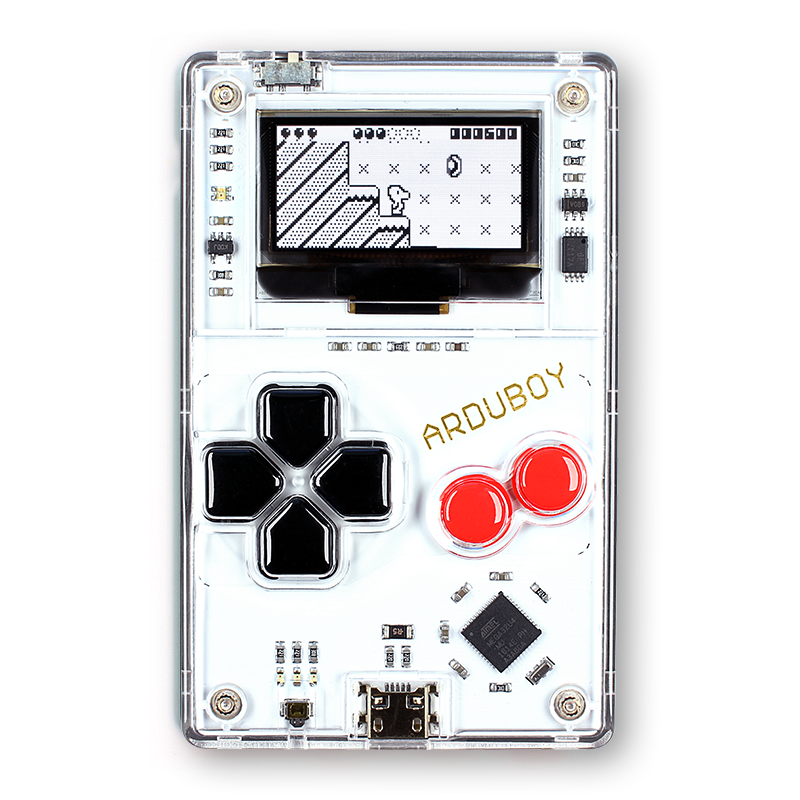
\includegraphics[width=13.4cm]{ArduboyGame.png}
\end{figure}

\section{Instellingen}
\label{sec:arduboy-instellingen}
% Arduino Leonardo
% Importeren library

Voor we aan de slag kunnen gaan met het programmeren van spelletjes voor de Arduboy, moeten we eerst enkele instellingen aanpassen in de Arduino IDE. Voor een handleiding met screenshots kan je terecht bij de Arduboy Community~\cite{arduboy:tuto1}.

\subsection{Installeren van de Arduboy2 library}
De \emph{Arduboy2} library bevat een handige interface die er voor zorgt dat we gemakkelijk alle functies van het apparaat kunnen aanspreken. Zo kunnen we ons volledig focussen op het ontwerpen en programmeren van het spel zelf. \\

\noindent
Alvorens we deze library kunnen gebruiken, moet ze eerst geïnstalleerd worden in de IDE. Dit doe je als volgt:

\begin{enumerate}
	\item Klik op \textbf{Hulpmiddelen} > \textbf{Bibliotheken beheren...}
	\item In het venster \emph{Bibliotheek Beheer} zoek je naar de library \textbf{Arduboy2}
	\item Installeer de laatste versie door de \textbf{Arduboy2} library aan te duiden en op \textbf{Installeren} te klikken
\end{enumerate}
Via deze manier kan je ook andere libraries installeren indien je dat wenst.

\subsection{Installeren van de Arduboy als Arduino board}
\begin{enumerate}
	\item Ga naar \textbf{Bestand} > \textbf{Voorkeuren}
	\item In het scherm \emph{Voorkeuren} geef je bij \textbf{Additionele Board Beheer URLs} de volgende URL in: \url{https://arduboy.github.io/board-support/package_arduboy_index.json}
	\item Klik op OK om het venster \emph{Voorkeuren} te sluiten
	\item Ga naar \textbf{Hulpmiddelen} > \textbf{Board} > \textbf{Board Beheer...}
	\item Zoek naar \textbf{Arduboy} en klik op \textbf{Installeren}
\end{enumerate}

\subsection{Board selecteren}
Om de IDE te laten weten dat je gaat programmeren voor de Arduboy, moet je het board in de IDE aanpassen. Ga naar \textbf{Hulpmiddelen} > \textbf{Board} en kies \textbf{Arduboy} in deze lijst.

\section{Programmastructuur}
\index{Programmastructuur}

\begin{minted}{cpp}
#include <Arduboy2.h>

Arduboy2 arduboy;

void setup() {
  arduboy.begin();
}

void loop() {
  if (arduboy.nextFrame()) {
    arduboy.clear();

    // GAME LOGIC
    
    arduboy.display();   
  }
}
\end{minted}
\noindent
Bovenstaand codefragment geeft een template van waar je kan starten om een Arduboy game te programmeren. Op de eerste lijn wordt de Arduboy2 library ingeladen. Daarna wordt er een \texttt{Arduboy2}-object aangemaakt. Dit object wordt gebruikt om de functionaliteit van de library op te roepen. In de \texttt{setup()} procedure wordt de functionaliteit van de Arduboy geïnitialiseerd. 

\section{De Arduboy2 library}
\index{Library}
Hier geven we een overzicht van de belangrijkste functies in de Arduboy2 library~\cite{arduboy:lib2-doc}. Deze functies kunnen op deze manier gebruikt worden:

\begin{center}
	\texttt{arduboy.functienaam();}
\end{center}
\noindent
Optionele parameters voor de functies staan \emph{schuingedrukt}.

\subsection{Init}
Deze functies worden gebruikt om de functionaliteit van de Arduboy te initialiseren.

\begin{libf}[begin()]
	Initialiseer de hardware, het logo weergeven, etc. Deze functie moet één keer opgeroepen worden in de \texttt{setup()} procedure.
\end{libf}

\begin{libf}[initRandomSeed()]
	Kies een random waarde als \emph{seed} voor de random number generator. Deze methode is het meest effectief wanneer ze na een (semi-)random tijd wordt opgeroepen.
\end{libf}

\subsection{Display}
Deze functies hebben betrekking tot het scherm van de Arduboy.

\begin{libf}[\textsc{Display}]
	Er zijn de volgende handige constanten voor de breedte en de hoogte van het scherm. Daarnaast zijn er ook constanten voor de kleuren van het scherm.
	\begin{multicols}{2}
		\begin{itemize}
			\item \texttt{WIDTH}
			\item \texttt{HEIGHT}
			\item \texttt{BLACK}
			\item \texttt{WHITE}
		\end{itemize}
	\end{multicols}
\end{libf}

\begin{libf}[clear()]
	Wis de display buffer. Het volledige scherm wordt op zwart gezet.
\end{libf}

\begin{libf}[display()]
	Plaats de inhoud van de display buffer op het scherm.
\end{libf}

\begin{libf}[setFrameRate(fps)]
	Stel de frame-rate in.\\ \\
	\textbf{Parameter}
	\begin{itemize}
		\item \texttt{int fps}: de gewenste frame-rate in frames per seconde
	\end{itemize}
\end{libf}

\begin{libf}[nextFrame()]
	Geeft aan of het tijd is om het volgende frame weer te geven.\\ \\
	\textbf{Returns}
	\begin{itemize}
		\item \texttt{bool}: \texttt{true} als het tijd is voor het volgende frame, anders \texttt{false}
	\end{itemize}
\end{libf}

\subsubsection{Draw}
Deze functies worden gebruikt om zelf vormen te tekenen op het scherm van de Arduboy.

\begin{libf}[drawPixel(x, y, \emph{color=WHITE})]
	Kleur een enkele pixel in de opgegeven kleur.\\ \\
	\textbf{Parameters}
	\begin{itemize}
		\item \texttt{int x}: x-coördinaat van de pixel
		\item \texttt{int y}: y-coördinaat van de pixel
		\item \texttt{int color} (optioneel): kleur $\rightarrow$ \texttt{WHITE} of \texttt{BLACK}
	\end{itemize}
\end{libf}

\begin{libf}[drawCircle(x, y, r, \emph{color=WHITE})]
	Teken een cirkel.\\ \\
	\textbf{Parameters}
	\begin{itemize}
		\item \texttt{int x}: x-coördinaat van het middelpunt van de cirkel
		\item \texttt{int y}: y-coördinaat van het middelpunt van de cirkel
		\item \texttt{int r}: straal van de cirkel
		\item \texttt{int color} (optioneel): kleur $\rightarrow$ \texttt{WHITE} of \texttt{BLACK}
	\end{itemize}
\end{libf}

\begin{libf}[drawRect(x, y, w, h, \emph{color=WHITE})]
	Teken een rechthoek.\\ \\
	\textbf{Parameters}
	\begin{itemize}
		\item \texttt{int x}: x-coördinaat van de linkerbovenhoek
		\item \texttt{int y}: y-coördinaat van de linkerbovenhoek
		\item \texttt{int w}: breedte
		\item \texttt{int h}: hoogte
		\item \texttt{int color} (optioneel): kleur $\rightarrow$ \texttt{WHITE} of \texttt{BLACK}
	\end{itemize}
\end{libf}

\begin{libf}[drawRoundRect(x, y, w, h, r, \emph{color=WHITE})]
	Teken een rechthoek met afgeronde hoeken.\\ \\
	\textbf{Parameters}
	\begin{itemize}
		\item \texttt{int x}: x-coördinaat van de linkerbovenhoek
		\item \texttt{int y}: y-coördinaat van de linkerbovenhoek
		\item \texttt{int w}: breedte
		\item \texttt{int h}: hoogte
		\item \texttt{int r}: straal van de afronding
		\item \texttt{int color} (optioneel): kleur $\rightarrow$ \texttt{WHITE} of \texttt{BLACK}
	\end{itemize}
\end{libf}

\begin{libf}[drawTriangle(x0, y0, x1, y1, x2, y2, \emph{color=WHITE})]
	Teken een driehoek.\\ \\
	\textbf{Parameters}
	\begin{itemize}
		\item \texttt{int x0, int x1, int x2}: x-coördinaten van de hoeken
		\item \texttt{int y0, int y1, int y2}: y-coördinaten van de hoeken
		\item \texttt{int color} (optioneel): kleur $\rightarrow$ \texttt{WHITE} of \texttt{BLACK}
	\end{itemize}
\end{libf}

\newpage

\begin{libf}[drawLine(x0, y0, x1, y1, \emph{color=WHITE})]
	Teken een lijn tussen de opgegeven punten.\\ \\
	\textbf{Parameters}
	\begin{itemize}
		\item \texttt{int x0, int x1}: x-coördinaten van de punten
		\item \texttt{int y0, int y1}: y-coördinaten van de punten
		\item \texttt{int color} (optioneel): kleur $\rightarrow$ \texttt{WHITE} of \texttt{BLACK}
	\end{itemize}
\end{libf}

\begin{libf}[drawFastVLine(x, y, h, \emph{color=WHITE})]
	Teken een verticale lijn.\\ \\
	\textbf{Parameters}
	\begin{itemize}
		\item \texttt{int x}: x-coördinaat van het bovenste uiteinde
		\item \texttt{int y}: y-coördinaat van het bovenste uiteinde
		\item \texttt{int h}: lengte
		\item \texttt{int color} (optioneel): kleur $\rightarrow$ \texttt{WHITE} of \texttt{BLACK}
	\end{itemize}
\end{libf}

\begin{libf}[drawFastHLine(x, y, w, \emph{color=WHITE})]
	Teken een horizontale lijn.\\ \\
	\textbf{Parameters}
	\begin{itemize}
		\item \texttt{int x}: x-coördinaat van het linkse uiteinde
		\item \texttt{int y}: y-coördinaat van het linkse uiteinde
		\item \texttt{int w}: lengte
		\item \texttt{int color} (optioneel): kleur $\rightarrow$ \texttt{WHITE} of \texttt{BLACK}
	\end{itemize}
\end{libf}

\begin{libf}[fillCircle(x, y, r, \emph{color=WHITE})]
	Teken een opgevulde cirkel.\\ \\
	\textbf{Parameters}
	\begin{itemize}
		\item \texttt{int x}: x-coördinaat van het middelpunt van de cirkel
		\item \texttt{int y}: y-coördinaat van het middelpunt van de cirkel
		\item \texttt{int color} (optioneel): kleur $\rightarrow$ \texttt{WHITE} of \texttt{BLACK}
	\end{itemize}
\end{libf}

\begin{libf}[fillRect(x, y, w, h, \emph{color=WHITE})]
	Teken een opgevulde rechthoek.\\ \\
	\textbf{Parameters}
	\begin{itemize}
		\item \texttt{int x}: x-coördinaat van de linkerbovenhoek
		\item \texttt{int y}: y-coördinaat van de linkerbovenhoek
		\item \texttt{int w}: breedte
		\item \texttt{int h}: hoogte
		\item \texttt{int color} (optioneel): kleur $\rightarrow$ \texttt{WHITE} of \texttt{BLACK}
	\end{itemize}
\end{libf}

\pagebreak

\begin{libf}[fillRoundRect(x, y, w, h, r, \emph{color=WHITE})]
	Teken een opgevulde rechthoek met afgeronde hoeken.\\ \\
	\textbf{Parameters}
	\begin{itemize}
		\item \texttt{int x}: x-coördinaat van de linkerbovenhoek
		\item \texttt{int y}: y-coördinaat van de linkerbovenhoek
		\item \texttt{int w}: breedte
		\item \texttt{int h}: hoogte
		\item \texttt{int r}: straal van de afronding
		\item \texttt{int color} (optioneel): kleur $\rightarrow$ \texttt{WHITE} of \texttt{BLACK}
	\end{itemize}
\end{libf}

\begin{libf}[fillTriangle(x0, y0, x1, y1, x2, y2, \emph{color=WHITE})]
	Teken een opgevulde driehoek.\\ \\
	\textbf{Parameters}
	\begin{itemize}
		\item \texttt{int x0, int x1, int x2}: x-coördinaten van de hoeken
		\item \texttt{int y0, int y1, int y2}: y-coördinaten van de hoeken
		\item \texttt{int color} (optioneel): kleur $\rightarrow$ \texttt{WHITE} of \texttt{BLACK}
	\end{itemize}
\end{libf}

\begin{libf}[fillScreen(\emph{color=WHITE})]
	Vul het scherm op met de opgegeven kleur.\\ \\
	\textbf{Parameters}
	\begin{itemize}
		\item \texttt{int color} (optioneel): kleur $\rightarrow$ \texttt{WHITE} of \texttt{BLACK}
	\end{itemize}
\end{libf}

\subsubsection{Text}
Deze functies worden gebruikt om tekst weer te geven op het scherm van de Arduboy.

\begin{libf}[setCursor(x, y)]
	Stel de locatie van de tekst cursor in.\\ \\
	\textbf{Parameters}
	\begin{itemize}
		\item \texttt{int x}: x-coördinaat
		\item \texttt{int y}: y-coördinaat
	\end{itemize}
\end{libf}

\begin{libf}[setTextSize(s)]
	Stel de grootte van de tekstkarakters in.\\ \\
	\textbf{Parameter}
	\begin{itemize}
		\item \texttt{int s}: tekstgrootte ($\geq 1$)
	\end{itemize}
\end{libf}

\begin{libf}[setTextColor(c)]
	Stel de tekstkleur in.\\ \\
	\textbf{Parameter}
	\begin{itemize}
		\item \texttt{int c}: kleur $\rightarrow$ \texttt{WHITE} of \texttt{BLACK}
	\end{itemize}
\end{libf}

\begin{libf}[setTextBackground(bg)]
	Stel de achtergrondkleur van de tekst in.\\ \\
	\textbf{Parameter}
	\begin{itemize}
		\item \texttt{int bg}: achtergrondkleur $\rightarrow$ \texttt{WHITE} of \texttt{BLACK}
	\end{itemize}
\end{libf}

\begin{libf}[setTextWrap(w)]
	Schakel text wrapping in of uit. Als text wrapping is ingeschakeld wordt de tekst op een nieuwe lijn geplaatst als deze te lang is om op de huidige lijn te passen.\\ \\
	\textbf{Parameter}
	\begin{itemize}
		\item \texttt{bool w}: \texttt{true} om text wrapping in te schakelen, \texttt{false} om uit te schakelen
	\end{itemize}
\end{libf}

% https://mlxxxp.github.io/documents/Arduino/libraries/Arduboy2/Doxygen/html/classPrint.html
\begin{libf}[\href{https://mlxxxp.github.io/documents/Arduino/libraries/Arduboy2/Doxygen/html/classPrint.html}{print(content)}]
	Print de opgegeven content op de plaats van de cursor.\\ \\
	\textbf{Parameter}
	\begin{itemize}
		\item \texttt{content}: tekst die weergegeven moet worden
	\end{itemize}
\end{libf}

\subsection{Buttons}
Met deze functies kan je interacties via de knoppen van de Arduboy programmeren.

\begin{libf}[\textsc{Buttons}]
	Voor de knoppen op de Arduboy zijn de volgende constanten gedefinieerd.
	\begin{multicols}{3}
		\begin{itemize}
			\item \texttt{A\_BUTTON}
			\item \texttt{B\_BUTTON}
			\item \texttt{LEFT\_BUTTON}
			\item \texttt{RIGHT\_BUTTON}
			\item \texttt{UP\_BUTTON}
			\item \texttt{DOWN\_BUTTON}
		\end{itemize}
	\end{multicols}
	
	Buttons kunnen samengevoegd worden in een mask: \texttt{LEFT\_BUTTON + A\_BUTTON}
\end{libf}

\begin{libf}[pressed(buttons)]
	Test of de opgegeven knoppen ingedrukt worden.\\ \\
	\textbf{Parameters}
	\begin{itemize}
		\item \texttt{int buttons}: een bit-mask die aangeeft welke knoppen getest moeten worden 
	\end{itemize}
	\textbf{Returns}
	\begin{itemize}
		\item \texttt{bool}: \texttt{true} als alle knoppen in het opgegeven mask momenteel ingedrukt zijn
	\end{itemize}
\end{libf}

\begin{libf}[notPressed(buttons)]
	Test of de opgegeven knoppen \textbf{niet} ingedrukt worden.\\ \\
	\textbf{Parameters}
	\begin{itemize}
		\item \texttt{int buttons}: een bit-mask die aangeeft welke knoppen getest moeten worden
	\end{itemize}
	\textbf{Returns}
	\begin{itemize}
		\item \texttt{bool}: \texttt{true} als alle knoppen in het opgegeven mask momenteel \textbf{niet} ingedrukt zijn
	\end{itemize}
\end{libf}

\newpage

\subsection{Physics}
Deze functies worden gebruikt om interacties tussen verschillende objecten in je game te berekenen.

\begin{libf}[collide(rect1, rect2)]
	Controleer of twee rechthoeken elkaar snijden.\\ \\
	\textbf{Parameters}	
	\begin{itemize}
		\item \texttt{Rect rect1, Rect rect2}: rechthoeken $\rightarrow$ Rect(int x, int y, int width, int height)
	\end{itemize}
	\textbf{Returns}
	\begin{itemize}
		\item \texttt{bool}: \texttt{true} als de opgegeven rechthoeken overlappen
	\end{itemize}
\end{libf}

\begin{libf}[collide(point, rect)]
	Controleer of een punt binnen een rechthoek ligt.\\ \\
	\textbf{Parameters}
	\begin{itemize}
		\item \texttt{Point point}: punt $\rightarrow$ Point(int x, int y)
		\item \texttt{Rect rect}: rechthoek $\rightarrow$ Rect(int x, int y, int width, int height)
	\end{itemize}
\end{libf}

\subsection{LED}
Via deze functies kan je de RGB LED van de Arduboy aansturen.

\begin{libf}[setRGBled(red, green, blue)]
	Stel de helderheid van de verschillende kleuren in de RGB LED in. De RGB LED zijn eigenlijk kleine individuele rode, groene en blauwe LEDs die zeer dicht bij elkaar geplaatst zijn. Door de helderheid van de 3 kleuren aan te passen, kan je verschillende kleuren tonen. 	
	De helderheid van elke LED kan een waarde aannemen van 0 (volledig uit) tot 255 (volledig aan).\\ \\
	\textbf{Parameters}
	\begin{itemize}
		\item \texttt{int red}: rode component
		\item \texttt{int green}: groene component
		\item \texttt{int blue}: blauwe component
	\end{itemize}
\end{libf}

\begin{libf}[setRGBled(color, val)]
	Stel de helderheid van één van de kleuren in, zonder de andere kleuren aan te passen.\\ \\
	\textbf{Parameters}
	\begin{itemize}
		\item \texttt{int color}: naam van de kleur: \texttt{RED\_LED}, \texttt{GREEN\_LED} of \texttt{BLUE\_LED}
		\item \texttt{int val}: helderheid, waarde tussen 0 en 255
	\end{itemize}
\end{libf}

\newpage
\section{Emulator}
\index{Emulator}
Als je een game aan het programmeren bent, wil je natuurlijk ook kunnen testen of deze werkt op de manier dat jij wil. Daarom bestaan er emulators voor de Arduboy.

\subsection{ProjectABE}
\href{https://felipemanga.github.io/ProjectABE/}{ProjectABE (\texttt{https://felipemanga.github.io/ProjectABE/})} is een online emulator voor de Arduboy.
Je kan je eigen game testen door op het startscherm onder \textbf{My Projects} > \textbf{New Game} te klikken. In het volgende scherm zie je de emulator, zoals in Figuur~\ref{fig:projectabe}.
\begin{wrapfigure}{r}{5.5cm}
	\centering
	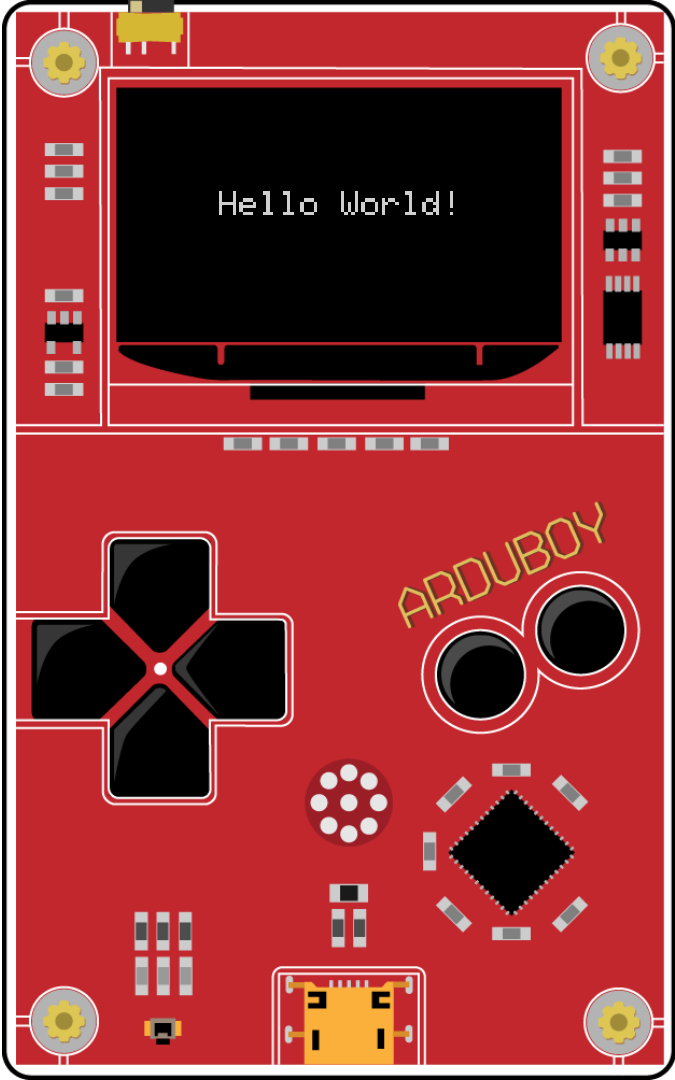
\includegraphics[width=5cm]{assets/ProjectABE}
	\caption{Project ABE}
	\label{fig:projectabe}
\end{wrapfigure}
% export binary
In de Arduino IDE klik je vervolgens op \textbf{Schets} > \textbf{Exporteer gecompileerd Binair bestand}. Hierdoor zal er een bestand met extensie \texttt{.hex} aangemaakt worden in dezelfde map als je code. Dit bestand met extensie \texttt{.hex} sleep je dan naar de emulator. De emulator zal dan meteen jouw code uitvoeren.\\
Je kan de emulator bedienen met het toetsenbord of door te klikken op de knoppen op het scherm.

\section{Programma op Arduboy plaatsen}
Voor je het programma op de Arduboy plaatst, controleer je best of zeker het juiste board staat geselecteerd (zie Sectie~\ref{sec:arduboy-instellingen}). Daarna zet je de Arduboy aan en verbind je hem met de computer via de USB-kabel. Vervolgens selecteer je de juiste poort via \textbf{Hulpmiddelen} > \textbf{Poort} en kies dan de optie waar Arduino bij staat.\\
Nu ben je volledig klaar om het programma op de Arduboy te plaatsen. Nu moet je enkel nog op het pijltje (\textbf{Uploaden}) klikken en even wachten. Als alles goed gaat staat je programma nu op de Arduboy.\\ \\
\emph{Veel gameplezier!}


%----------------------------------------------------------------------------------------
%	BIBLIOGRAPHY
%----------------------------------------------------------------------------------------

\chapterimage{jcw_header.pdf}

\chapter*{Bibliografie}
\addcontentsline{toc}{chapter}{\textcolor{ocre}{Bibliografie}} % Add a Bibliography heading to the table of contents

\printbibliography[heading=bibempty]

%----------------------------------------------------------------------------------------
%	INDEX
%----------------------------------------------------------------------------------------

\cleardoublepage % Make sure the index starts on an odd (right side) page
\phantomsection
\setlength{\columnsep}{0.75cm} % Space between the 2 columns of the index
\addcontentsline{toc}{chapter}{\textcolor{ocre}{Index}} % Add an Index heading to the table of contents
\printindex % Output the index

%----------------------------------------------------------------------------------------

\end{document}
